\documentclass[a4paper]{scrartcl}

% Font and Language
\usepackage{graphicx}
\usepackage{longtable}
\usepackage[utf8]{inputenc}
\usepackage[T1]{fontenc}
\usepackage[english]{babel}
\usepackage{lmodern}
\usepackage{amsmath}
\usepackage{float}

\usepackage{hyperref}
\KOMAoptions{fontsize=12pt}
\KOMAoptions{parskip=off}

\usepackage[
	left=2.5cm,
	right=2.5cm,
	top=2.5cm,
	bottom=4.5cm
]{geometry}

\usepackage[backend=biber]{biblatex}
\usepackage{csquotes}
\addbibresource{references.bib}

\usepackage{blindtext}

\usepackage[headsepline,footsepline]{scrlayer-scrpage}

\newcommand{\paperTitle}{Smart Climate and Air \\ 
Quality Control Systems}
\title{\paperTitle}
\clearpairofpagestyles
\rehead{\paperTitle}
\rohead{\paperTitle}

\newcommand{\paperAuthor}{Bhartkumar Boricha, Utkarsh Singh, \\ Romil Khokhani, Alikhan Begzhan, Numan Tasaddaq}
\author{
    Bhartkumar Boricha~<b.boricha@stud.fh-sm.de>, 313905\\
    Utkarsh Singh~<u.singh@stud.fh-sm.de>, 313870\\
    Romil Khokhani~<r.khokhani@stud.fh-sm.de>, 313903\\
    Alikhan Begzhan~<a.begzhan@stud.fh-sm.de>, 312542\\
    Numan Tasaddaq~<n.tasaddaq@stud.fh-sm.de>, 319414 \\
}

\lehead{\paperAuthor}
\lohead{\paperAuthor}

\usepackage{lastpage}
\refoot{\thepage{}~of~\pageref{LastPage}}
\rofoot{\thepage{}~of~\pageref{LastPage}}

\usepackage{graphicx}
\KOMAoptions{footheight=3cm}
\lefoot{\vspace*{1.3in}
\includegraphics[height=1cm]{images/suas-logo}}
\lofoot{
\includegraphics[height=1.5cm]{images/suas-logo}}

\cfoot{\href{https://github.com/AlikhanBegzhan/Smart-Climate-and-Air-Quality-Control-System-on-Pinecone-BL602}{\textbf{GitHub Repository}}}

\date{}

\begin{document}
	\maketitle

\begin{abstract}
    \section*{Abstract}
		Smart climate and air quality control systems are transforming indoor environments by using IoT, advanced sensors, and automation to optimize temperature, humidity and air quality. These systems monitor pollutants like CO and enhance energy efficiency, creating healthier and more sustainable spaces. This report examines a modular IoT-enabled system powered by the PineCone1 microcontroller, which uses sensors such as DHT22 and MQ-2. Features include self-sufficient functioning, secure data transmission, and user-friendly interfaces. Increased usage in residential, healthcare, and urban settings demonstrate scalability and adaptability, while emerging technologies like machine learning and smart city integration can be used to further improve their effectiveness. Despite challenges such as sensor calibration and data privacy, these systems offer significant potential for health, energy savings, and sustainability.
\end{abstract}
    
\section{Introduction}
Smart homes are becoming increasingly popular as technology advances, offering convenience and enhanced living experiences. However, these luxuries often come with a hefty price tag due to the sophisticated and complex technology they require, the cost of installation, and the need for regular maintenance. \cite{r4}\cite{r9} One essential component of smart homes is Air Quality monitoring technology, which has been widely used across industries such as food processing, healthcare and pharmaceuticals, and smart cities and urban development, etc. In the context of smart homes, temperature sensors play a pivotal role in smart climate and air quality control systems. These sensors are reliable, accurate, and versatile, providing several advantages such as reducing energy costs, improving appliance safety, and increasing heating or cooling efficiency depending on the circumstances. By integrating temperature monitoring into smart home setups,\cite{r10} homeowners can monitor energy consumption, regulate temperature effectively, and enhance overall energy efficiency. Amidst an energy procurement crisis, especially in regions like Europe, such systems have become increasingly critical. Smart climate control systems equipped with temperature sensors can optimize the operation of gas-based heaters, enabling users to save significant energy costs while reducing emissions that harm the environment. These systems ensure heaters operate only when necessary, preventing overuse and maintaining desired temperatures, thereby conserving energy and resources. Modern smart systems go beyond temperature regulation by integrating air quality control features to detect and address harmful gases like CO2.\cite{r11} By automating ventilation and providing real-time alerts, these systems promote healthier indoor environments while dynamically adjusting heating, cooling, and ventilation based on real-time data. Advanced sensors optimize temperature, humidity, and air quality, seamlessly integrating with home automation to enhance energy efficiency and sustainability. This dual focus on climate and air quality creates more sustainable, efficient, and eco-friendly living spaces. These IoT-enabled technologies are transforming indoor environmental management, making homes smarter, greener, and more comfortable while ensuring safety and health. The system is versatile, serving homes, schools, and healthcare facilities by maintaining ideal conditions for comfort, learning, and patient care. Its scalability and adaptability make it a key component in smart city development, enhancing urban living standards while supporting climate change mitigation and resource efficiency.\cite{r13}
\section{Goals and Objective}
This project focuses on enhancing human living conditions by enhancing indoor air quality and monitoring the system using IoT to improve health and energy efficiency. By leveraging real-time sensors and developing smart automation, the system ensures optimal temperature, humidity, and air quality, reducing health risks associated with poor ventilation and pollutants such as asthma, bronchitis, and other respiratory diseases. Maintaining a healthy indoor environment leads to better sleep, improved cognitive function, and overall well-being. Additionally, intelligent energy management minimizes excessive heating or cooling, reducing energy consumption and costs. By integrating IoT-driven monitoring, this project aims to create a sustainable and health-focused living space while optimizing energy efficiency.

\section{Literature Review}
According to the European Commission, research suggests that humans spend approximately 85-90\% of their lives indoors \cite{r19}. This highlights the significant impact that indoor environments have on our health, well-being, and overall quality of life. Given this, factors like indoor air quality, lighting, and ventilation play a crucial role in maintaining a healthy lifestyle.

Smart homes equipped with indoor air quality (IAQ) management systems represent a transformative approach to creating healthier and more sustainable living environments. By integrating interconnected sensors, automation, and real-time analytics, these systems optimize indoor conditions such as temperature, humidity, and air quality while addressing pollutants like carbon dioxide (CO2). Originally centered on energy efficiency, modern smart home technologies now prioritize IAQ management to mitigate health risks, such as respiratory issues and cognitive impairments, which are aggravated by poor air quality and environmental pollution.

Studies have highlighted the effectiveness of these systems, with Fisk emphasizing their role in mitigating health risks linked to climate change, particularly for vulnerable populations \cite{r14}. Similarly, Wallner et al \cite{r3}. demonstrated that mechanical ventilation systems in energy-efficient homes maintain better IAQ compared to naturally ventilated homes, especially in urban settings where exposure to outdoor pollutants is higher . Additionally, Kumar et al . showed how demand-driven, data-responsive ventilation systems in smart homes not only improve IAQ but also significantly reduce energy consumption \cite{r2}. 

Recent advancements in this field include IoT-enabled multi-sensor networks, which provide affordable and accessible real-time monitoring of IAQ metrics, and predictive analytics powered by machine learning, which can anticipate air quality fluctuations and adjust climate controls proactively. These technologies now extend their applications beyond residential spaces to include schools, where they promote healthier learning environments, and healthcare facilities, where they support infection control and enhance patient care. The integration of IAQ systems with Ambient Assisted Living (AAL) solutions has also expanded their scope to include health tracking for elderly populations, showcasing their potential in specialized healthcare contexts \cite{r2}

Furthermore, smartphone integration allows users to remotely monitor IAQ and receive alerts, offering greater convenience and control. Despite these advancements, challenges remain. A significant research gap lies in the lack of standardized protocols for IAQ sensors, resulting in inconsistent data accuracy across different environments. Moreover, the integration of IAQ systems with broader urban environmental monitoring frameworks is still underexplored, despite its relevance in densely populated areas where outdoor air quality concerns are prominent.

While existing studies underscore the short-term health benefits of improved IAQ, there is a need for longitudinal research to assess the sustained impacts, particularly for children, the elderly, and other vulnerable groups. Additionally, debates persist over the extent of automation versus user control in these systems, with some users preferring manual adjustments despite the proven benefits of automated optimization. Data privacy and security also remain critical concerns, as IAQ systems collect detailed information about home environments and occupant behaviors, necessitating robust safeguards against unauthorized access \cite{r16}. 

In conclusion, smart home technologies integrated with IAQ management systems hold immense potential to revolutionize indoor climate control and promote healthier, more sustainable living spaces. However, addressing challenges like sensor standardization, urban integration, and privacy concerns is crucial for unlocking their full potential. These systems not only enhance individual health and well-being but also contribute to broader goals like climate change mitigation, urban sustainability, and the development of smart cities. By advancing research and addressing current limitations, smart IAQ systems can play a pivotal role in shaping a future where indoor environments are healthier, safer, and more efficient.

Maintaining an optimal room temperature is crucial for enhancing sleep quality, cognitive function, and overall longevity. Research indicates that both excessively high and low ambient temperatures can impair cognitive performance, particularly in older adults. A study utilizing data from the Chinese Longitudinal Healthy Longevity Survey found that for each 1\,°C increase in high monthly temperatures, global cognitive function scores decreased by 0.48 points, while a 1\,°C decrease in low temperatures resulted in a 0.14-point decline. This suggests that high temperatures have a more pronounced negative effect on cognitive abilities \cite{r21}. 

Furthermore, sleep quality is intricately linked to cognitive performance. Research involving older adults from six middle-income countries demonstrated that better sleep quality and intermediate sleep durations are associated with enhanced cognitive functions, including memory and attention \cite{r24}. Additionally, maintaining regular sleep patterns has been identified as a stronger predictor of reduced mortality risk compared to sleep duration alone. A prospective cohort study revealed that consistent sleep schedules significantly lower the risk of all-cause mortality \cite{r22}.

In summary, maintaining a comfortable room temperature supports better sleep quality, which in turn enhances cognitive function and may contribute to increased longevity.

In another research paper, we found that the integration of Internet of Things (IoT) technologies has revolutionized traditional environmental monitoring by giving rise to advanced smart climate and air quality control systems, which autonomously regulate indoor environments to enhance occupant comfort, health, and safety. These systems rely on IoT-enabled sensors and microcontrollers to monitor and adjust critical parameters such as temperature, humidity, and pollutant levels in real time, ensuring a balanced and optimized indoor atmosphere\cite{r23}.

For example, systems like the Smart Climate and Air Quality Control System use a network of sensors, including the DHT22 for humidity and temperature monitoring, alongside CO2 and CO gas sensors for detecting air pollutants, providing detailed environmental data that is essential for maintaining healthy conditions. The core objectives of these systems include improving air quality, maintaining thermal comfort, and enhancing energy efficiency by making adjustments only when necessary.

Automation plays a central role in these systems, using real-time data processing to activate devices such as air purifiers, heaters, and humidifiers, ensuring optimal environmental conditions with minimal energy consumption. Additionally, user interaction is facilitated through intuitive interfaces like smartphone apps, allowing users to monitor and adjust system settings, view real-time environmental data, and receive alerts.

This level of user engagement ensures that the system is customized to meet individual needs, improving user satisfaction. However, despite the benefits, IoT-based climate control systems face several challenges. Sensor calibration and data accuracy remain significant concerns, as low-cost sensors can experience calibration drift, leading to inaccuracies in pollutant level measurements. Regular recalibration is needed to maintain system performance, especially in applications where precise monitoring of pollutants is critical.

Moreover, power management is a key issue in battery-operated systems, necessitating the development of energy-efficient protocols and optimized sampling rates to extend system longevity. Looking ahead, emerging trends in IoT-based climate control systems include the use of machine learning algorithms to predict and adjust climate parameters proactively, based on historical data and environmental conditions.

These advancements can enhance system responsiveness to fluctuations in air quality, providing more effective climate management. Furthermore, integrating these systems into smart city infrastructures offers vast potential for community-wide health and environmental monitoring. By collecting and analyzing data on both indoor and outdoor air quality, these systems can support urban planning, public health initiatives, and environmental policy-making.

In conclusion, IoT-based smart climate and air quality control systems present a transformative solution for creating healthier and more sustainable indoor environments. With ongoing advancements in sensor accuracy, machine learning, and energy-efficient technologies, these systems are poised to play a crucial role in improving indoor air quality, reducing energy consumption, and promoting overall well-being. Future developments in sensor reliability, smart city integration, and energy efficiency will continue to expand the impact of these systems, enabling smarter, healthier, and more sustainable urban living spaces.
\section{Research Questions}
\begin{enumerate}
    \item How can IoT technology enhance real-time monitoring and control of indoor conditions, specifically temperature, humidity, and air quality?
    \item What configurations and placements of sensors are most effective for accurate, continuous data collection in indoor environments?
    \item How efficiently does the PineCone1 microcontroller process data from multiple environmental sensors to support real-time system responses?
    \item What impact does user customization, such as setting environmental thresholds, have on user satisfaction and system adaptability?
    \item How critical is ongoing sensor calibration to maintaining the accuracy and reliability of environmental data over time?
    \item How effectively does the system’s modular design support scalability for additional sensors or devices?
    \item What cybersecurity risks exist for IoT-based climate control systems, and how can these be minimized?
    \item How does real-time data visualization on mobile and web platforms improve user interaction and control over indoor environmental conditions?
\end{enumerate}

\section{Methodology}

\subsection{System Architecture}
The Smart Climate and Air Quality Control System is designed with a structured and modular architecture, ensuring efficient real-time monitoring and control of indoor environmental conditions. The architecture consists of multiple layers:

\begin{itemize}
\item \textbf{Sensing Layer:} The system employs the DHT22 sensor to measure temperature and humidity, while the MQ2 sensor detects air quality by identifying gases such as CO, LPG, and smoke. These sensors continuously collect real-time environmental data.
\item \textbf{Processing Layer:} The PineCone1 microcontroller serves as the system's core, processing data received from the sensors. It executes decision-making algorithms based on predefined threshold values and triggers the appropriate actuators accordingly.
\item \textbf{Actuation Layer:} To regulate indoor climate, the system uses an Arctic P12 PC fan for ventilation and a PTC fan heater for temperature control. These actuators are controlled by the microcontroller via a 2-channel relay module.
\item \textbf{Communication Layer:} The system implements the TCP/IP protocol over Wi-Fi, ensuring secure and efficient data exchange between the microcontroller and the web interface. This allows users to monitor and control the system remotely.
\item \textbf{User Interface Layer:} A web-based dashboard provides real-time visualization of sensor readings and system status. Users can manually control the fan and heater or allow the system to operate autonomously.
\item \textbf{Power Supply Layer:} The system is powered by a 12V 12A power supply, with a USB DC-DC buck converter ensuring stable voltage regulation for various components.
\end{itemize}

\subsection{Hardware and Software Selection}

\subsubsection{Hardware Components}
\begin{itemize}
\item \textbf{Sensors:}
\begin{itemize}
\item \textbf{DHT22:} Measures temperature and humidity with high precision.
\item \textbf{MQ2:} Detects gases such as CO, LPG, and smoke for air quality monitoring.
\end{itemize}
\item \textbf{Microcontroller:} PineCone1, selected for its efficiency and Wi-Fi capability.
\item \textbf{Actuators:}
\begin{itemize}
\item \textbf{Arctic P12 PC Fan:} Provides cooling and air circulation.
\item \textbf{PTC Fan Heater:} Generates heat to maintain optimal indoor temperatures.
\end{itemize}
\item \textbf{Control Module:} 2-channel relay module for switching actuators on and off.
\item \textbf{Power Management:}
\begin{itemize}
\item \textbf{USB DC-DC Buck Converter:} Regulates voltage as required.
\item \textbf{12V 12A Power Supply:} Ensures reliable operation.
\end{itemize}
\end{itemize}

\subsubsection{Software Components}
\begin{itemize}
\item \textbf{Programming Language:} C, chosen for its efficiency in embedded systems development.
\item \textbf{Development Tools:}  Bouffalo lab software sdk for writing, compiling, and uploading firmware to the PineCone1 microcontroller.
\item \textbf{Communication Protocol:}TCP/IP for real-time and secure data exchange over Wi-Fi.
\item \textbf{User Interface:} Web-based dashboard for remote monitoring and control.
\end{itemize}

\subsection{Development Process}

\subsubsection{Requirement Analysis}
\begin{itemize}
\item Define system objectives, constraints, and performance criteria.
\item Identify sensor thresholds for temperature, humidity, and air quality.
\item Determine user requirements for web interface functionality.
\end{itemize}

\subsubsection{Hardware Integration}
\begin{itemize}
\item Connect sensors to the PineCone1 microcontroller.
\item Interface actuators (fan and heater) with the 2-channel relay module.
\item Set up power connections using the 12V 12A supply and buck converter.
\end{itemize}

\subsubsection{Firmware Development}
\begin{itemize}
\item Write C-based firmware to read sensor data and process it.
\item Implement logic for controlling the fan and heater based on sensor readings.
\item Use of HTTP for data transmission to the web interface.
\end{itemize}

\subsubsection{Web Interface Development}
\begin{itemize}
\item Develop a web dashboard to display real-time temperature, humidity, and air quality data.
\item Implement controls for manually operating the fan and heater.
\item Enable remote monitoring via a user-friendly interface.
\end{itemize}

\subsubsection{System Optimization}
\begin{itemize}
\item Optimize sensor data collection and filtering to reduce noise values.
\item Improve power efficiency to extend device lifespan.
\item Implement security measures like wifi  for secure communication.
\end{itemize}

\subsection{Testing and Validation}

\subsubsection{Component Testing}
Each hardware component is tested individually:
\begin{itemize}
\item DHT22 and MQ2 sensors are verified for accuracy.
\item The microcontroller's processing capability is assessed.
\item The fan and heater are checked for proper functionality.
\end{itemize}

\subsubsection{Firmware Testing}
\begin{itemize}
\item The C code is tested for bugs and optimized for efficiency.
\item Data transmission is validated.
\item The relay module's response time is measured.
\end{itemize}

\subsubsection{Integration Testing}
\begin{itemize}
\item The interaction between sensors, the microcontroller, and actuators is tested.
\item Communication with the web interface is verified.
\item The system's ability to handle different environmental conditions is evaluated.
\end{itemize}

\subsubsection{System Performance Testing}
\begin{itemize}
\item Response time is measured to ensure real-time operation.
\item The system's stability under prolonged usage is tested.
\item The power consumption of the entire system is analyzed.
\end{itemize}

\subsubsection{User Testing}
\begin{itemize}
\item The web interface is tested for usability and responsiveness.
\item Users interact with the system to provide feedback on ease of use and reliability.
\end{itemize}

\subsubsection{Final Validation}
\begin{itemize}
\item Ensures compliance with system requirements.
\item Confirms reliability, accuracy, and efficiency before deployment.
\end{itemize}


\section{Hardware Setup}
The Smart Climate and Air Quality Control System is designed with an efficient hardware setup that enables real-time monitoring and control of indoor climate conditions. The system consists of sensors for data collection, actuators for temperature regulation, a microcontroller for processing, and a power supply to ensure stable operation.

\subsection{System Components}
The system integrates multiple hardware components, each playing a crucial role in data acquisition, processing, and climate regulation. Below is a breakdown of each component.

\subsubsection{Pinecone BL602 Microcontroller}
The Pinecone BL602 is the central processing unit of the system, responsible for handling sensor data and controlling actuators. It is a low-power, Wi-Fi-enabled microcontroller that allows real-time communication with the web-based user interface.

\textbf{Key Features:}
\begin{itemize}
    \item Processor: RISC-V-based BL602 SoC (System on Chip)
    \item Memory: 128KB RAM (limitation in handling large processes)
    \item Connectivity: Supports Wi-Fi 2.4 GHz for remote monitoring
    \item Programming: Uses C/C++ for firmware development
    \item GPIO: Controls sensors, relay module, and power supply components
\end{itemize}

\textbf{Limitations:}
\begin{itemize}
    \item Limited onboard storage
    \item Requires external storage or processing unit (e.g., Raspberry Pi) for advanced functionalities \cite{r15}
\end{itemize}

Pinecone BL602 collects temperature, humidity, and gas concentration data from the DHT22 and MQ2 sensors and processes this information to make control decisions. Based on the analysis, it activates or deactivates the Arctic P12 fans and PTC heaters through the relay module.

\subsubsection{DHT22 Temperature and Humidity Sensor}
The DHT22 sensor is responsible for monitoring temperature and humidity in the indoor environment. It provides digital output and operates with low power consumption \cite{r1}.

\textbf{Specifications:}
\begin{itemize}
    \item Temperature range: -40°C to 80°C
    \item Accuracy: ±0.5°C
    \item Humidity range: 0-100\% RH
    \item Humidity accuracy: ±2\% RH
    \item Sampling rate: Once every 2 seconds
\end{itemize}

\textbf{Functionality in the Project:}
DHT22 is connected to Pinecone BL602, which reads the temperature and humidity values. If the humidity exceeds the set threshold, the cooling fans activate to improve air circulation. If the temperature is too high or too low, the system either turns on the fans or activates the heater to maintain optimal indoor conditions.

\subsubsection{MQ2 Gas Sensor}
The MQ2 gas sensor is used to detect harmful gases such as carbon monoxide (CO), propane, butane, and methane \cite{r12}. It provides an analog output, which is processed by the Pinecone BL602 to determine the gas concentration.

\textbf{Specifications:}
\begin{itemize}
    \item Detection range: 200 – 10,000 ppm
    \item Sensitivity: High to LPG, propane, and hydrogen gases
    \item Response time: ≤10 seconds
    \item Operating voltage: 5V
\end{itemize}

\textbf{Functionality in the Project:}
If gas leakage is detected, the system immediately alerts the user via the web interface. If gas levels exceed the safe threshold, the Arctic P12 fans activate to improve ventilation. The system ensures that air pollutants are managed effectively, preventing health risks.

\subsubsection{Arctic P12 PWM PST Fans}
The Arctic P12 PWM PST fans provide air circulation and cooling to regulate temperature and humidity. These fans are energy-efficient and designed for silent operation \cite{r8}.

\textbf{Specifications:}
\begin{itemize}
    \item Voltage: 12V
    \item Airflow: 56.3 CFM
    \item Power Consumption: 0.08A
    \item Noise Level: Low (≤23.5 dB)
\end{itemize}

\textbf{Functionality in the Project:}
The fans are controlled via a relay module, allowing automatic activation/deactivation based on environmental conditions. When the humidity exceeds the threshold, the fans activate to remove excess moisture. When the temperature is too high, the fans cool the environment by circulating air. If high gas concentration is detected, the fans improve ventilation by dispersing harmful gases.

\subsubsection{PTC Fan Heater}
The PTC (Positive Temperature Coefficient) fan heater is used for heating the indoor environment when the temperature drops below a set threshold. Unlike traditional heaters, PTC heaters are self-regulating, meaning they automatically adjust their power consumption based on temperature changes \cite{r18}.

\textbf{Specifications:}
\begin{itemize}
    \item Voltage: 12V
    \item Power Consumption: 100W
    \item Current Draw: ~8.3A
    \item Safety Feature: Overheat protection
\end{itemize}

\textbf{Functionality in the Project:}
The PTC heater is connected to the relay module, which allows the Pinecone BL602 to turn it on/off based on temperature conditions. If the temperature falls below the user-defined threshold, the heater activates warming the indoor space. Once the temperature returns to the normal range, the heater turns off, preventing unnecessary power consumption.

\subsubsection{Power Supply and Relays}
The system requires a stable power source to operate all components effectively. It includes a 12V power supply \cite{r6}, a DAC converter (12V to 5V) \cite{r7} , and a relay \cite{r5} module for device control.

\textbf{Power Supply Specifications:}
\begin{itemize}
    \item Voltage: 12V
    \item Current: 12A (capable of handling system’s max 9A consumption)
\end{itemize}

\textbf{Functionality:}
The power supply ensures stable operation of the fans, heaters, and sensors. The system consumes approximately 9A, while the power supply provides 12A, ensuring a safe margin for power efficiency.

The DAC converter steps down 12V to 5V to power the Pinecone BL602 safely, preventing damage to the microcontroller by ensuring it does not receive excess voltage.

The relay module acts as a switch to control the fans and heater. The Pinecone BL602 sends a 5V signal to the relay, which activates/deactivates the connected devices.

\subsection{Circuit Diagram and Explanation}
The circuit diagram illustrates the connections between sensors, the microcontroller, the relay module, and the power supply.
\begin{figure}[H]
    \centering
    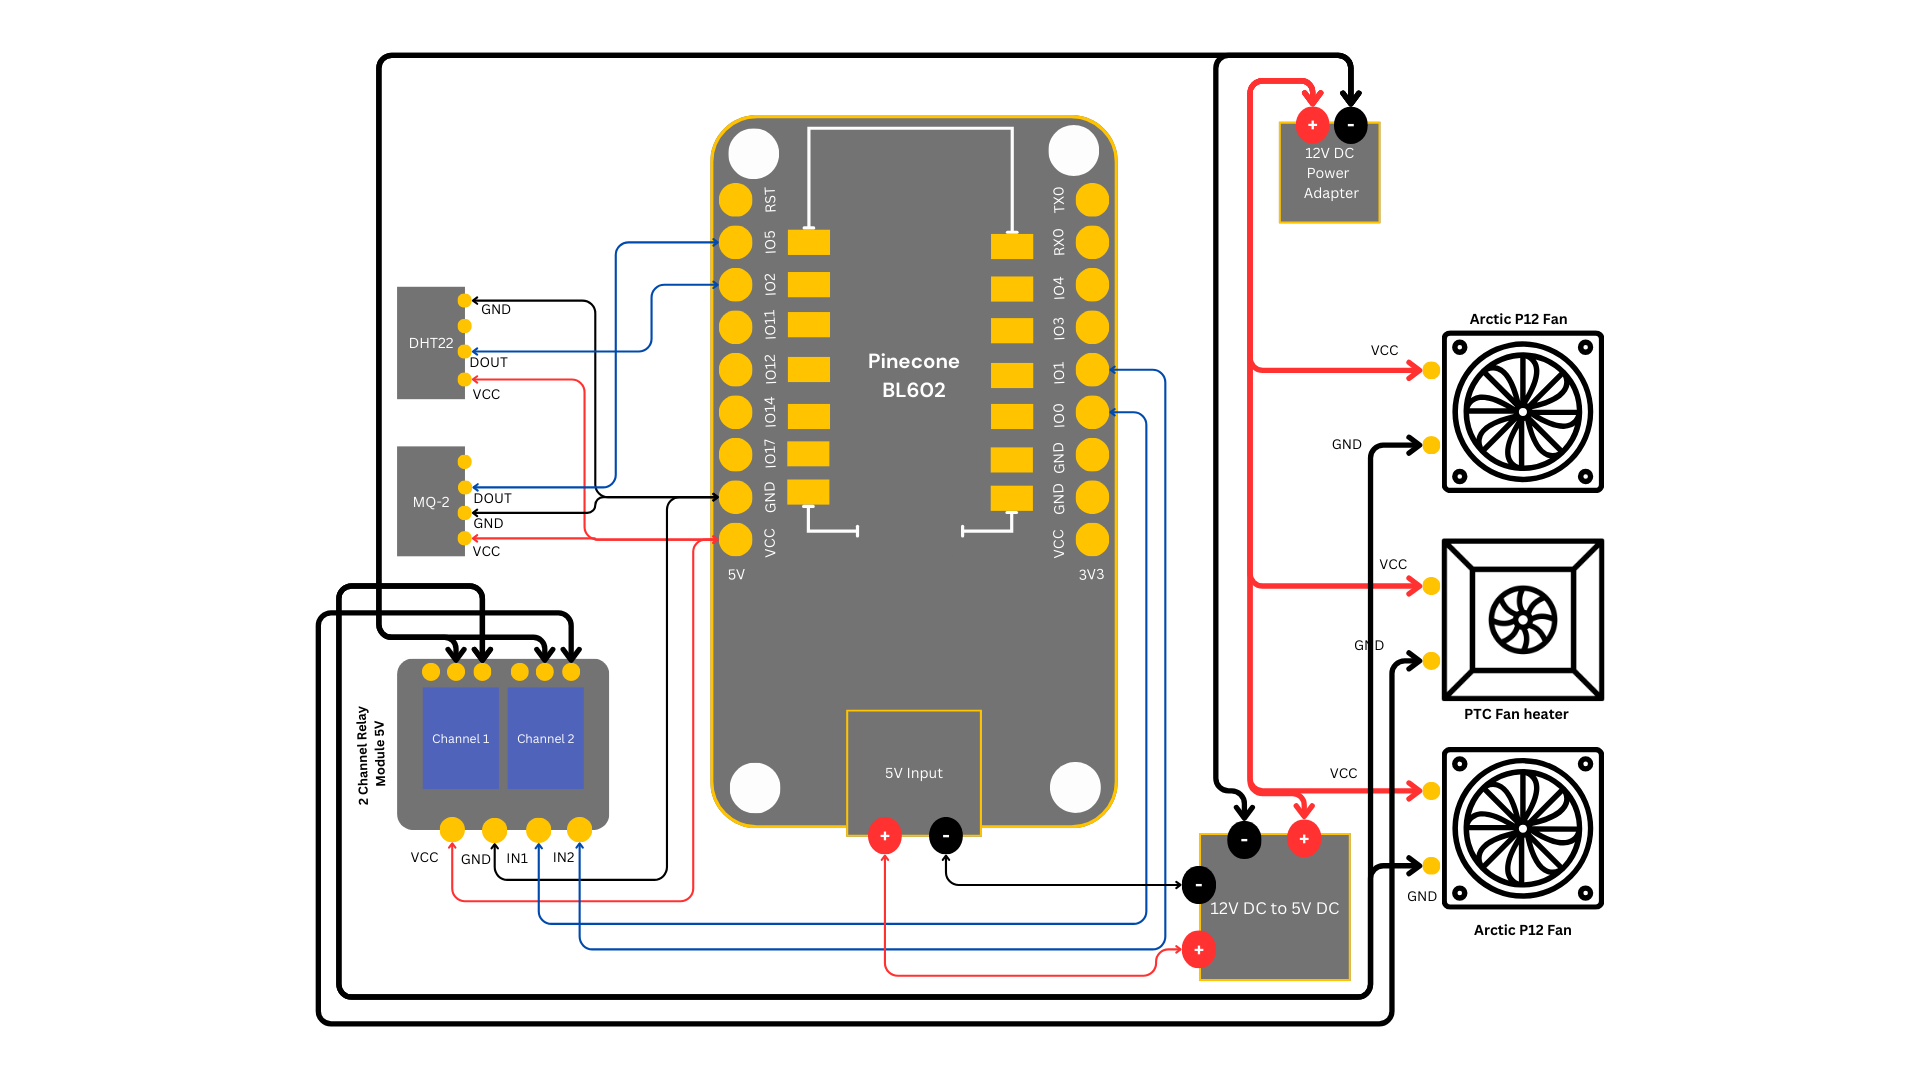
\includegraphics[width=1\textwidth]{images/CD.png}
    \caption{Circuit Diagram}
\end{figure}

\subsubsection{Explanation of Circuit Components and Connections}
\begin{enumerate}
    \item \textbf{Pinecone BL602 Microcontroller}
    \begin{itemize}
        \item Power Source: Connected to a 5V supply via a DAC (12V to 5V converter) to prevent damage.
        \item Sensor Inputs: DHT22 sensor connected to a digital GPIO pin; MQ2 sensor provides analog output connected to an ADC-compatible pin.
    \end{itemize}
    
    \item \textbf{Relay Module (2-Channel, 5V)}
    \begin{itemize}
        \item Connected to two GPIO pins of the Pinecone BL602 and acts as a switching mechanism for the Arctic P12 Fans and PTC Heater.
    \end{itemize}
    
    \item \textbf{Actuators (Fans and Heater)}
    \begin{itemize}
        \item Arctic P12 Fans connected to Relay Output 1; PTC Fan Heater connected to Relay Output 2.
    \end{itemize}
    
    \item \textbf{Power Supply and DAC Converter}
    \begin{itemize}
        \item 12V, 12A Power Supply supplies power to fans, heater, and DAC converter.
        \item DAC Converter steps down voltage for safe operation.
    \end{itemize}
    
    \item \textbf{Wi-Fi Communication for Web Interface}
    \begin{itemize}
        \item The Pinecone BL602 connects to a Wi-Fi router and runs an HTTP server for user interaction.
    \end{itemize}
\end{enumerate}

\subsection{Hardware Assembly and Configuration}
\begin{enumerate}
    \item {Connected the Sensors (DHT22 \& MQ2) to the Pinecone BL602}
    \item {Wiring the Relay Module to the Pinecone BL602}
    \item {Connecting Actuators (Fans and Heater) to the Relay Module}
    \item {Power Supply Integration}
\end{enumerate}

\section{System Overview and Operation}
The Smart Climate and Air Quality Control System is designed to autonomously monitor, process, and regulate indoor environmental conditions. The system architecture ensures seamless communication between sensors, controllers, and actuators, with user access through a web interface for real-time monitoring and manual control.

\subsection{System Architecture}
The system follows modular architecture, allowing efficient interaction between hardware components, data processing units, and the user interface.

\subsubsection{Block Diagram}
\begin{figure}[H]
    \centering
    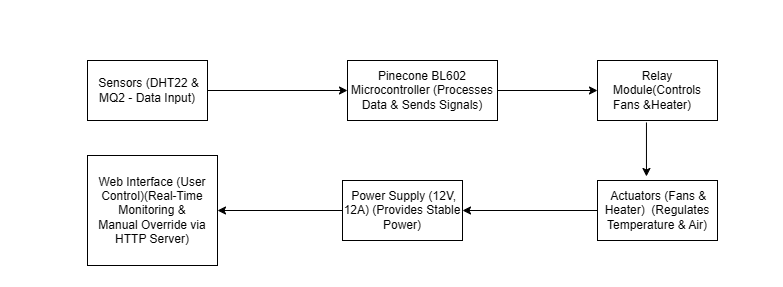
\includegraphics[width=1\textwidth]{images/BD.png}
    \caption{Block Diagram}
\end{figure}

The block diagram consists of the following major components:
\begin{itemize}
    \item Sensors (DHT22 \& MQ2) → Data Acquisition
    \item Pinecone BL602 Microcontroller → Data Processing \& Control
    \item Relay Module → Actuator Control
    \item Power Supply (12V, 12A) → System Power Management
    \item Web Interface → User Interaction
\end{itemize}

\subsection{System Workflow}
The system follows a real-time monitoring and response mechanism to ensure a safe and comfortable indoor environment. The workflow involves data collection, processing, decision-making, and user interaction through a web interface.

\subsection{Data Acquisition and Processing}
\subsubsection{Data Acquisition}
The system continuously collects real-time data from the DHT22 and MQ2 sensors.

\subsubsection{Data Processing}
The Pinecone BL602 microcontroller continuously receives sensor readings, compares them with preset thresholds, and activates fans or heaters if limits are exceeded.

\subsection{Control Mechanisms}
The system has two modes of operation: Automated Control Mode and Manual Control Mode. 

\subsubsection{User Interface}
The Smart Climate and Air Quality Control System includes a web-based interface that allows users to monitor real-time data, adjust settings, and manually control devices.

\section{Web Interface Features}
The web interface consists of three key sections: Data Monitoring, Limit Setting, and Fan Controls.

\begin{figure}[H]
    \centering
    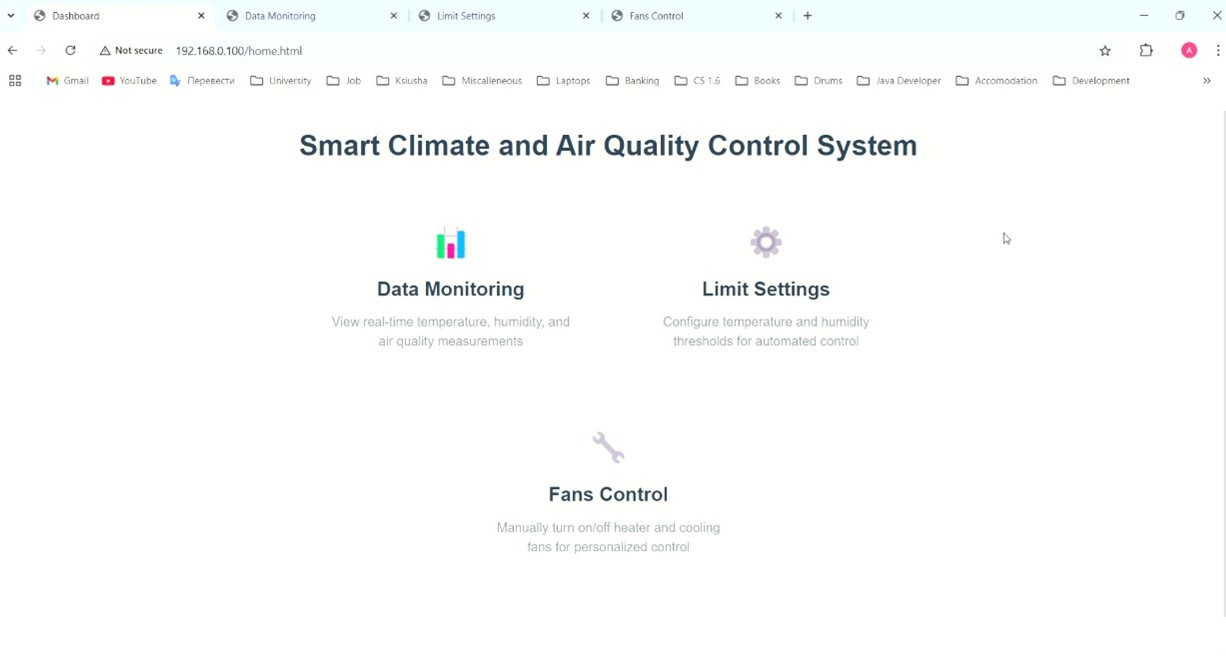
\includegraphics[width=0.8\textwidth]{images/HP.jpg}
    \caption{Home Page}
\end{figure}

\subsection{ Data Monitoring Tab}
Displays real-time sensor data, including:
\begin{itemize}
    \item Temperature (°C)
    \item Humidity (%)
    \item Gas Concentration (PPM)
\end{itemize}
Live data updates every 1-2 seconds to ensure accuracy. If gas levels exceed safety limits, a warning alert appears on the screen.

\begin{figure}[H]
    \centering
    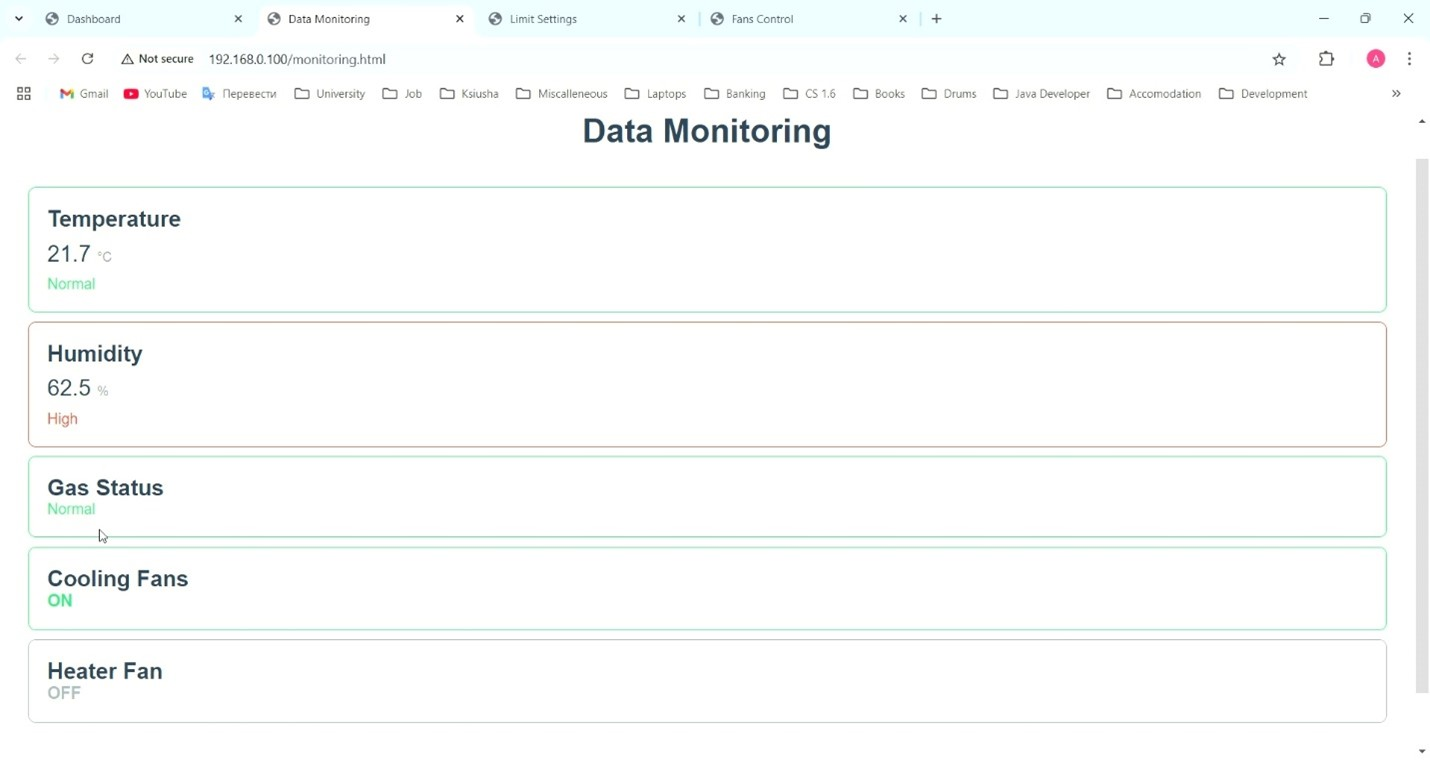
\includegraphics[width=0.8\textwidth]{images/DMP.jpg}
  \caption{Data monitoring Page}
\end{figure}



\subsection{ Limit Settings Tab}
Allows users to set custom thresholds for temperature and humidity. Includes safety checks:
\begin{itemize}
    \item Prevents setting high temperature limits lower than low temperature limits.
    \item Displays an error message if incorrect values are entered.
\end{itemize}
\begin{figure}[H]
    \centering
    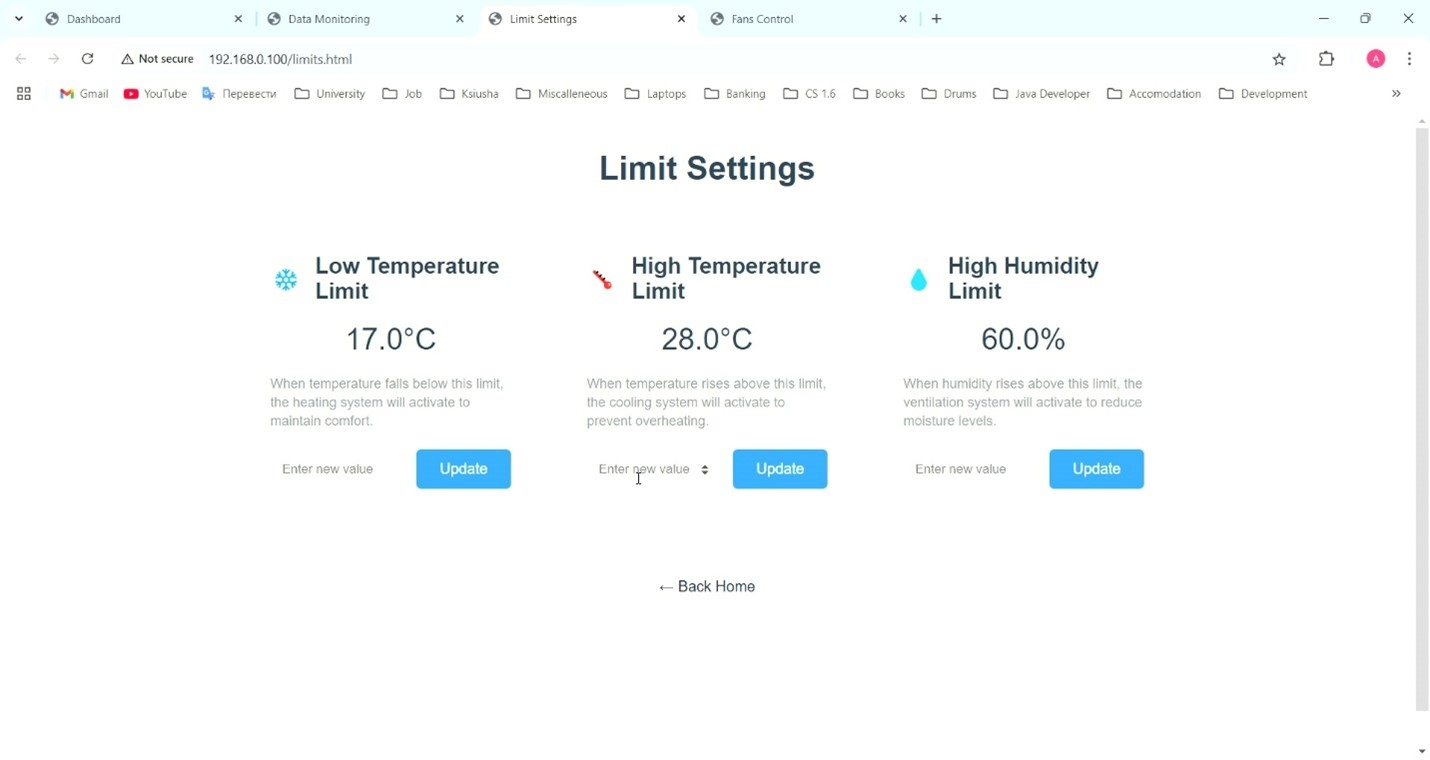
\includegraphics[width=0.8\textwidth]{images/LSP.jpg}
    \caption{Limit Setting Page}
\end{figure}



\subsection{ Fan \& Heater Control (Manual Mode)}
Users can manually control the system when necessary:
\begin{itemize}
    \item Turn ON/OFF fans regardless of temperature/humidity levels.
    \item Activate/deactivate the PTC heater manually.
    \item Enable or disable manual mode with a single button.
    \item Visual indicators show which devices are running currently.
\end{itemize}
\begin{figure}[H]
    \centering
    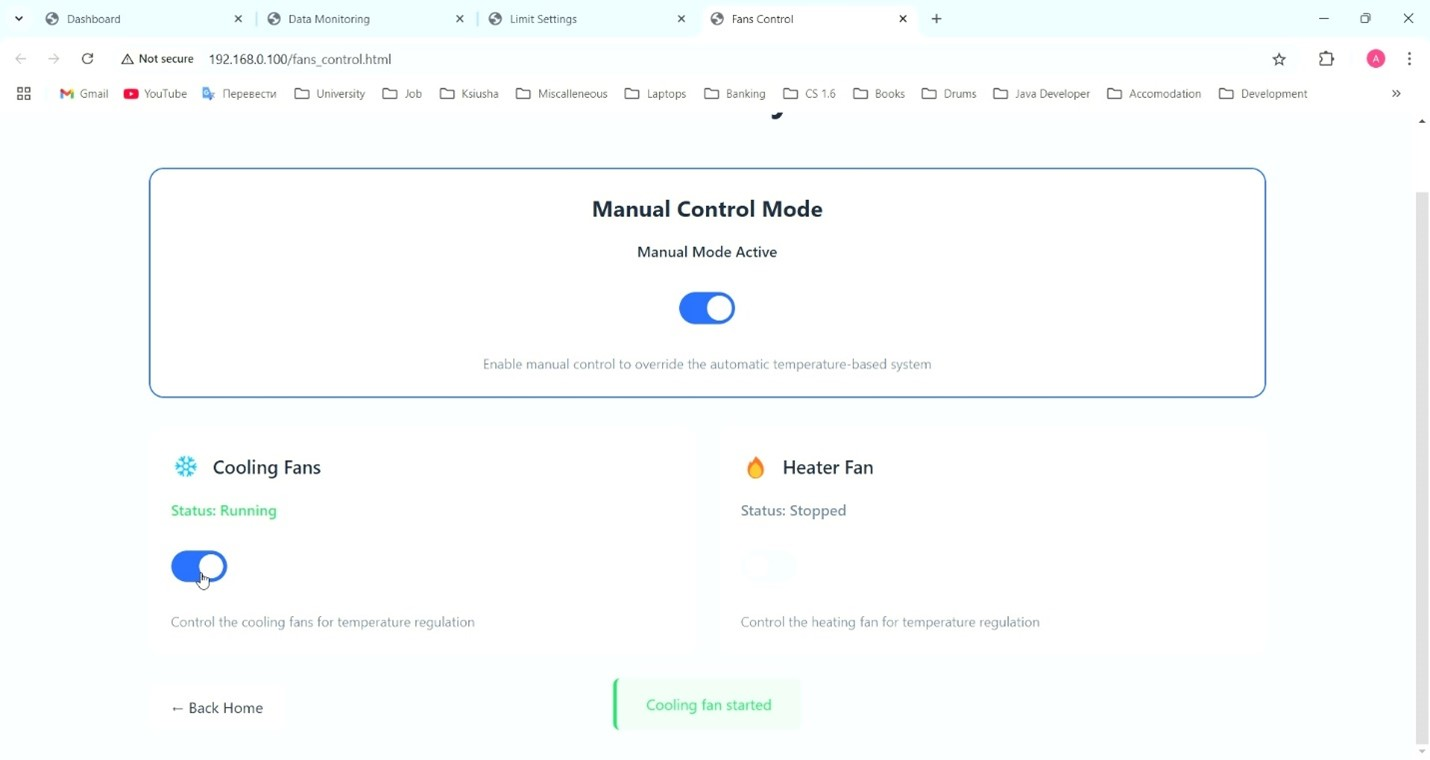
\includegraphics[width=0.8\textwidth]{images/MCP.jpg}
    \caption{Manual Mode Page}
\end{figure}


\subsection{Fan \& Heater Control (Automatic Mode)}
This is the default mode when the system is live, and the following actions are performed automatically according to the readings from sensors:
\begin{itemize}
    \item If temperature exceeds the high threshold, Arctic P12 cooling fans activate to regulate airflow.
    \item If humidity exceeds the threshold, fans improve air circulation to reduce moisture.
    \item If the temperature drops below the low threshold, the PTC heater turns ON. Once the temperature reaches the normal range, the heater turns OFF to prevent overheating.
    \item If the MQ2 sensor detects gas leakage, the system alerts the user via the web interface, and fans are turned ON to ventilate the area and disperse harmful gases.
\end{itemize}
\begin{figure}[H]
    \centering
    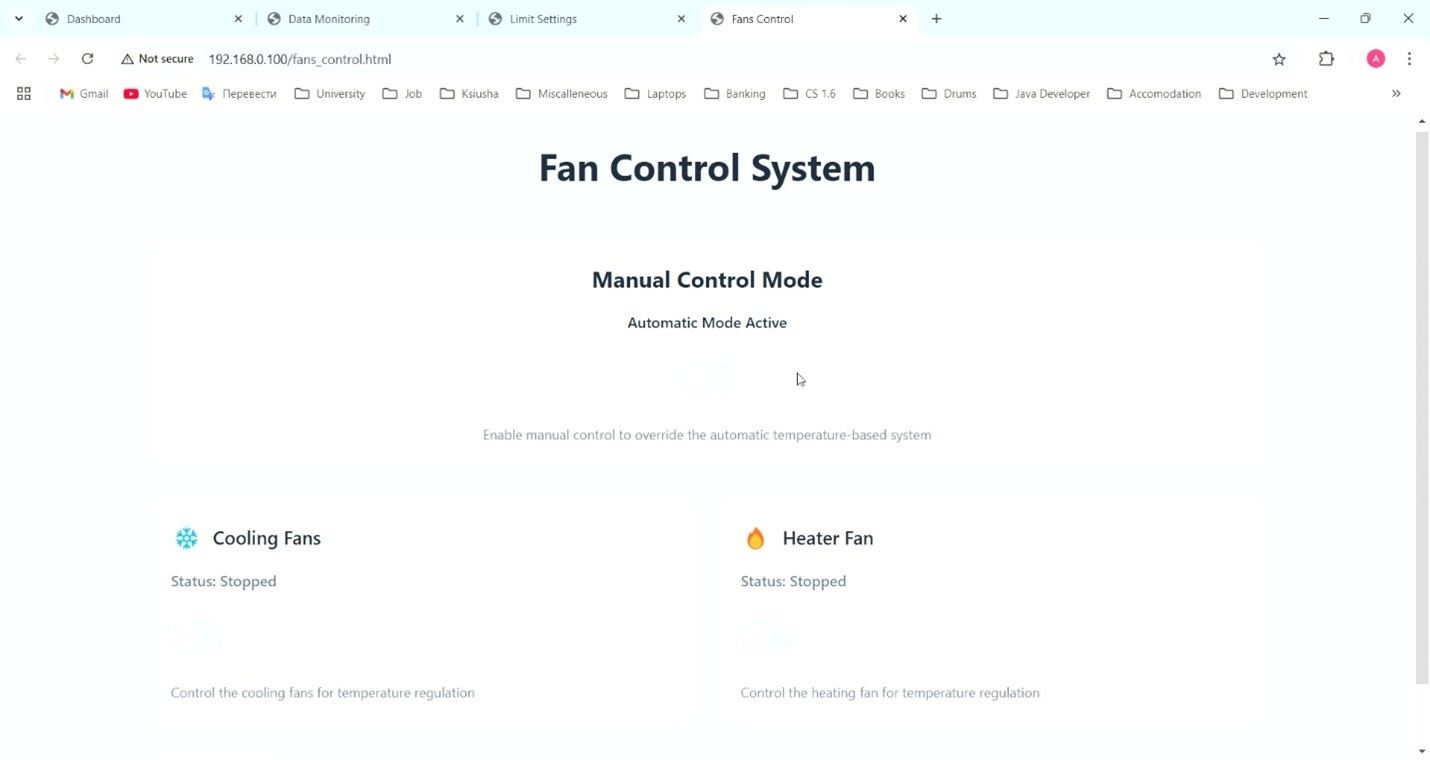
\includegraphics[width=0.8\textwidth]{images/AM.jpg}
    \caption{Automatic Mode Page}
\end{figure}


\subsection{Web Interface Connectivity}
The Pinecone BL602 hosts an HTTP server over a Wi-Fi network. Users can access the interface via a web browser on their phone, tablet, or PC. The system provides secure access with authentication features to prevent unauthorized control.



\section{Implementation Details}

\subsection{Software Implementation}
The software implementation of the Smart Climate and Air Quality Control System was designed to handle real-time data acquisition, processing, and control mechanisms. The firmware was developed using C programming for low-level microcontroller operations, ensuring efficient hardware utilization and real-time responsiveness.

\subsubsection{Firmware Development}
The firmware was developed specifically for the PineCone BL602 microcontroller, utilizing its built-in Wi-Fi and GPIO capabilities. The program continuously reads environmental data from the DHT22 temperature and humidity sensor and MQ2 gas sensor, processes this data, and executes predefined control actions. Threshold-based algorithms were implemented to trigger actuators such as the PTC fan heater and Arctic P12 PWM PST fans whenever environmental conditions exceeded predefined limits.

\subsubsection{Communication Protocols (TCP/IP)}
The system employs TCP/IP (Transmission Control Protocol/Internet Protocol) for reliable communication between the microcontroller and the web-based user interface. TCP/IP  ensures error-checked, connection-oriented data transmission, making it suitable for real-time sensor monitoring and control.

\paragraph{Data Transmission Process}
\begin{itemize}
    \item The PineCone BL602 establishes a TCP connection with a locally hosted user interface on home wifi/network.
    \item Sensor data is packetized and transmitted over the network using standard HTTP or WebSocket protocols running over TCP.
    \item The Javascript (on browser) processes the received data and updates the user dashboard in real-time.
\end{itemize}

\paragraph{Advantages of TCP/IP in the System}
\begin{itemize}
    \item \textbf{Reliable delivery}: Ensures sensor data reaches the localhost server without packet loss.
    \item \textbf{Error correction}: TCP/IP detects and retransmits lost packets, preventing missing or inaccurate readings.
    \item \textbf{Compatibility}: Easily integrates with existing IoT and cloud infrastructures without requiring an broker in future integration.
    \item \textbf{Real-time updates}: WebSockets over TCP allow continuous data streaming, reducing latency compared to traditional HTTP polling.
\end{itemize}

\subsubsection{Algorithm Design}
The control algorithm is based on threshold-based decision-making combined with feedback control. The key components of the algorithm include:
\begin{itemize}
    \item \textbf{Temperature Control}: If the room temperature falls below the set threshold, the PTC heater is activated.
    \item \textbf{Air Quality Control}: If Butane or other pollutants exceed safety limits, the fans are activated to improve ventilation.
    \item \textbf{Humidity Regulation}: If humidity is too high, the system starts the fans to maintain comfortable levels.
\end{itemize}

\subsection{Integration of Components}
The integration of hardware and software was achieved through serial communication protocols between the sensors and the PineCone BL602 microcontroller. The actuators were controlled using relay modules, allowing the system to operate in an automated manner. The integration process involved:
\begin{enumerate}
    \item Configuring the DHT22 sensor for continuous temperature and humidity monitoring.
    \item Ensuring the MQ2 sensor accurately detects gas concentrations and relays data to the microcontroller.
    \item Implementing relay switching mechanisms for activating fans and heaters based on environmental conditions.
    \item Developing a dashboard interface to display real-time sensor data and allow manual control.
\end{enumerate}

\subsection{Data Transmission and Security}
Security is a critical aspect of the implementation, especially in TCP/IP-based communication. Several measures were taken to ensure secure and efficient data transmission:
\begin{itemize}
    \item \textbf{TLS Encryption}: All TCP connections were secured using Transport Layer Security (TLS) to prevent man-in-the-middle (MITM) attacks.
    \item \textbf{Authentication Mechanism}: In future secure login credentials and API keys would be implemented to restrict unauthorized access to the system.
\end{itemize}






\section{Results}
The prototype is an IoT-based indoor air quality and environmental monitoring system which is designed to enhance both health and energy efficiency by automatically regulating temperature, humidity, and air quality within the environment. The system is centered around the Pinecone microcontroller, which acts as the primary control unit, processing data in real-time from two essential sensors: the DHT22 sensor, responsible for monitoring temperature and humidity levels, and the MQ2 gas sensor, which detects hazardous gases such as carbon monoxide, methane, and other volatile organic compounds. The continuous data feed allows the system to make intelligent decisions, ensuring a healthy indoor atmosphere by responding to environmental changes effectively. The microcontroller interacts with a two-channel relay module operating at five volts, which is responsible for controlling various output devices, including two Arctic P12 cooling fans and a PTC fan heater. These devices play a crucial role in maintaining the desired indoor conditions, responding to real-time sensor data and user-defined threshold values.

The Pinecone microcontroller processes the incoming data and triggers the relay module to either activate or deactivate this devices based on predefined thresholds. For example, if the humidity surpasses the set limit, the cooling fans are turned on to bring it back to normal levels. Similarly, if the temperature drops below a specified threshold, the PTC fan heater is activated to restore comfort. This automation ensures minimal human intervention while maintaining optimal environmental conditions. One of the critical aspects of the system is power management. To ensure stable and efficient operation, a 12V to 5V converter is incorporated, preventing damage to the microcontroller while ensuring sufficient power delivery. The entire system is powered by a dedicated power supply unit capable of delivering 12V at 12A, ensuring all components receive adequate power while maintaining energy efficiency by consuming less than 80 perc. of the power supply’s total capacity.

A significant feature of this project is its integration with an HTTP server, which is deployed by the Pinecone microcontroller and operates over a Wi-Fi network. This setup enables remote monitoring and control, providing users with an intuitive interface accessible via a web browser. 
The user interface consists of multiple tabs: data monitoring, limit settings, and fan control. 

The data monitoring page provides real-time updates on environmental parameters, including temperature, humidity, and gas concentration. The interface visually represents these values, allowing users to track changes over time. Additionally, an alert mechanism is implemented to notify users in case of critical changes, such as the detection of dangerous gas levels.

The limit settings page offers customization options, allowing users to set their preferred temperature and humidity thresholds. These adjustments ensure flexibility, catering to varying comfort preferences and environmental conditions. Importantly, the system includes safeguards to prevent incorrect configurations; for instance, it does not allow the user to set a high-temperature limit lower than the low-temperature limit. This ensures logical consistency in environmental control and prevents potential operational errors.
The fan control page provides an additional layer of flexibility by offering both automated and manual control options. While the system is designed to function autonomously, users can switch to manual mode and override automated operations if necessary. This feature is particularly useful in scenarios where immediate intervention is required, such as feeling excessively hot or cold despite automated adjustments. Users can also manually toggle the cooling fans and heater using simple button controls, enhancing the overall usability of the system.

To demonstrate the effectiveness of the system, several tests were conducted. The gas detection mechanism was validated by exposing the MQ2 sensor to a lighter’s gas emissions, which triggered an immediate alert on the user interface, confirming its ability to detect harmful gases in real time. Similarly, the humidity sensor's responsiveness was tested by applying moisture to the DHT22 sensor, which resulted in an observable increase in humidity levels on the data monitoring page, subsequently activating the cooling fans as per the set threshold. The temperature control mechanism was also tested by adjusting the limit settings and observing the activation and deactivation of the PTC heater and cooling fans accordingly. These tests confirm the system’s reliability and responsiveness in maintaining indoor air quality.

The project effectively demonstrates the advantages of IoT-based environmental monitoring and automation. By continuously monitoring indoor conditions and making real-time adjustments, the system significantly improves air quality, reducing health risks associated with poor ventilation, excessive humidity, and harmful gases. Furthermore, the integration of intelligent energy management ensures that devices are only activated when necessary, thereby optimizing power consumption and reducing overall energy costs. This makes the system a sustainable solution for residential, commercial, and industrial applications.

In conclusion, the IoT-based indoor air quality monitoring system presents a comprehensive solution for maintaining a healthy and energy-efficient indoor environment. Through the seamless integration of sensors, a microcontroller, relay-controlled devices, and an intuitive web-based interface, the project achieves both automation and user control. The system's ability to detect hazardous gases, regulate temperature and humidity, and provide remote monitoring makes it a valuable addition to modern smart home and building automation systems. Future enhancements could include additional sensors like humidifiers and other sensors that showcase more detailed environmental analysis, integration with smart home ecosystems, and the implementation of AI-driven predictive maintenance for even more efficient control. This project lays the foundation for further research and development in smart environmental control, contributing to healthier and more energy-efficient living spaces.

\section{Challenges and Solutions}

\subsection{Technical Challenges}
During the development and testing phases, several technical challenges were encountered, including:
\begin{enumerate}
    \item \textbf{Network Latency and TCP Overhead}
        \begin{itemize}
            \item TCP's handshake and acknowledgments introduced latency.
            \item Optimizing packet sizes and buffers reduced transmission delays.
            \item Congestion control caused delays under high traffic.
            \item Packet retransmissions affected real-time responsiveness.
            \item TCP's overhead made it less efficient than UDP for low-latency streaming.
            \item WebSockets improved TCP streaming but required fine-tuning.
        \end{itemize}
    \item \textbf{Sensor Calibration and Accuracy Issues}
       \begin{itemize}
    \item The MQ2 sensor readings varied due to humidity, temperature fluctuations, and sensor drift.  
    \item The DHT22 required frequent recalibration for accuracy.  
    \item External pollutants and electronic noise affected gas concentration readings.  
    \item Response times varied with environmental conditions, needing algorithm adjustments.  
    \item Lack of standardized calibration led to inconsistent accuracy, requiring real-time adjustments.  
    \item Sensor aging reduced reliability, necessitating periodic recalibration or replacement.  
\end{itemize}
    \item \textbf{Power Management and Energy Consumption}
    \begin{itemize}
    \item Continuous operation impacted power efficiency.  
    \item Wi-Fi communication required low-power modes.  
    \item Actuators needed optimized control to save power.  
    \item Microcontroller power use varied with network activity.  
    \item Frequent data transmission drained battery life.  
    \item Heat dissipation increased energy consumption.  
    \item Sleep modes and duty cycling were challenging.  
\end{itemize}
    \item \textbf{Firmware Debugging and Compatibility Issues}
     \begin{itemize}
    \item The BL602 required specific firmware configurations.  
    \item Driver issues caused occasional sensor data failures.  
    \item Memory limits required algorithm optimization.  
    \item Debugging async sensor failures was challenging.  
    \item Inconsistent SDK updates required regression testing.  
    \item Stack overflows needed better memory management.  
    \item Efficient interrupt handling added complexity.  
\end{itemize}

\end{enumerate}

\subsection{Solutions Implemented}
To address these challenges, the following solutions were implemented:
\begin{enumerate}
    \item \textbf{Optimized TCP/IP Communication}
        \begin{itemize}
            \item Reduced packet size and optimized buffer management to improve response time.
            \item Switched to WebSockets for faster, persistent connections, eliminating repeated TCP handshakes.
        \end{itemize}
    \item \textbf{Sensor Calibration and Accuracy Enhancements}
        \begin{itemize}
            \item Regular recalibration of DHT22 and MQ2 sensors was performed using reference devices to ensure data accuracy.
        \end{itemize}
    \item \textbf{Power Optimization Strategies}
        \begin{itemize}
            \item Energy-efficient relay modules were selected to minimize power wastage.
        \end{itemize}
    \item \textbf{Firmware Debugging and Compatibility Fixes}
        \begin{itemize}
            \item Compatibility issues with the PineCone BL602 were resolved by using an optimized device driver.
        \end{itemize}
\end{enumerate}

\subsection{Lessons Learned}
Throughout the development process, several key lessons were learned:
\begin{enumerate}
    \item \textbf{Optimizing TCP/IP for IoT Systems}
        \begin{itemize}
            \item While TCP/IP is reliable, its overhead must be minimized for real-time applications by optimizing data transmission intervals.
        \end{itemize}
    \item \textbf{Real-World Testing is Essential}
        \begin{itemize}
            \item Real-world testing in different environmental conditions helped identify network latency issues that were not evident in simulations.
        \end{itemize}
    \item \textbf{Scalability Considerations}
        \begin{itemize}
            \item Future enhancements should focus on modular design, allowing the addition of new sensors without significant reconfiguration.
        \end{itemize}
    \item \textbf{Security is a Priority}
        \begin{itemize}
            \item IoT-based systems must incorporate secure communication protocols (e.g., TLS, authentication tokens) to prevent unauthorized access.
        \end{itemize}
\end{enumerate}

\begin{center}
    \textbf{Table 1: Reviewer Feedback and How We Addressed It}
\end{center}

\begin{longtable}{|c|p{6cm}|p{6cm}|}
    \hline
    \textbf{No.} & \textbf{Reviewer Feedback} & \textbf{How We Addressed It} \\ 
    \hline
    1 & The paper lacks real-world experimental validation and quantitative performance metrics. & A miniature prototype with a web UI was developed to showcase real-world scenarios and quantitative metrics. \\ 
    \hline
    2 & More details on system scalability and adaptability to diverse environments are needed. & A detailed use case in the future scope discusses scalability and potential improvements with better resources. \\ 
    \hline
    3 & Sensor calibration issues and long-term reliability concerns should be addressed. & Sensor calibration issues were acknowledged in the final presentation, but long-term reliability remains an assumption. \\ 
    \hline
    4 & Data security measures beyond http need further elaboration. & Data security has been covered to the best extent possible in the report. \\ 
    \hline
    5 & User interface design and user interaction details require more emphasis. & UI design was demonstrated in the final presentation and included in the report. \\ 
    \hline
    6 & Comparative analysis with existing solutions should be included to highlight novelty. & A direct comparison wasn’t feasible due to the lack of an exact model for evaluation. \\ 
    \hline
    7 & A cost-benefit analysis would strengthen the feasibility argument. & The prototype cost around 120 euros; large-scale production would cost significantly more. \\ 
    \hline
    8 & Real-world case studies or deployment examples should be added. & Relevant research papers and related projects were included in the literature review. \\ 
    \hline
    9 & The methodology section needs enhancement with clearer rationale and testing procedures. & The methodology section has been revised and improved. \\ 
    \hline
    10 & Figures and diagrams require better annotation for clarity. & Annotations were improved in the latest version of the report. \\ 
    \hline
    11 & More references should be cited for stronger context and credibility. & Additional references were added throughout the report for better context. \\ 
    \hline
    12 & Challenges like sensor inaccuracies and power consumption should be mitigated with practical solutions. & A 12V power supply was used, and its impact was detailed in the recorded video and in the report. \\ 
    \hline
    13 & Language, formatting, and organization improvements are needed for better readability. & Final formatting and readability improvements were made in the project report. \\ 
    \hline
\end{longtable}

\section{Future Improvements}
Adopting machine learning is the way forward in the space of the IOT Sector. To achieve optimal temperature adjustment using machine learning, the process begins by collecting and analyzing vast amounts of historical temperature data. This data can include factors such as the time of day, day of the week, seasonal trends, local weather patterns, humidity levels, and geographical location.\cite{r20} Once the data is gathered, machine learning models, particularly supervised learning algorithms like linear regression, decision trees, or more advanced techniques like deep learning, are used to identify patterns and correlations within the data. For instance, the model could predict temperature fluctuations based on the time of day and season, understanding that temperature behavior at noon in winter will likely differ from noon in summer.

The system would use this model to continuously learn from incoming real-time data. For example, a smart thermostat in a home would adjust the temperature dynamically, not just based on preset schedules, but also in real-time, taking into account the changing weather conditions, time of day, and even the presence of people in the room. The model would predict the optimal temperature required, learning from its past adjustments and user preferences, which can be explicitly set or inferred by the system. It could also account for outside factors like energy usage, adjusting settings to ensure that it’s not just comfortable but also energy-efficient.

Adopting machine learning in temperature regulation provides numerous benefits to the user experience. The first advantage is personalization. Users will no longer need to manually adjust their systems as the model adapts to their preferences, whether they like a cooler room during the night or a warmer one in the morning. Over time, the system learns individual patterns of usage, adjusting itself for maximum comfort. Another key benefit is energy efficiency. By learning the most efficient times and settings to adjust the temperature, machine learning minimizes unnecessary energy consumption, resulting in lower utility bills and a reduced carbon footprint. 

Furthermore, this level of automation creates a more seamless, intuitive experience, where the user is freed from constantly monitoring and adjusting their home or office temperature.
Additionally, machine learning makes it possible to integrate with other IoT devices within the smart home ecosystem. For instance, a smart thermostat could collaborate with weather forecast systems, open/closed windows, or even occupancy sensors to create a fully integrated environment. This synergy between devices enhances the overall user experience, making the environment more comfortable and responsive to user behavior without requiring active intervention. The adaptability and continuous learning capabilities of machine learning make this system more intelligent over time, providing increasingly accurate predictions and adjustments, thus improving the system’s long-term effectiveness.

Another Use Case it to design a system where the temperature adapts to a user's body temperature when they enter a room from outside, It requires a combination of two sensors, one capturing outdoor air temperature and the other capturing indoor air temperature, it would be the foundation for smart environmental control. The outdoor sensor continuously monitors the ambient outdoor temperature, providing real-time data on the external weather conditions. The indoor sensor, installed within the room, continuously tracks the temperature inside the room, offering insights into how the room’s environment is reacting to external factors. However, to make the room adapt to the user’s body temperature upon entry, the system would incorporate an additional sensor, such as a thermal imaging sensor or infrared sensor, capable of detecting the user's body temperature when they cross the entry threshold. By analyzing the difference between the outdoor and indoor temperatures, combined with the user’s body heat, the system can intelligently adjust the room’s climate to optimize comfort. For instance, if a user enters from a hot or cold external environment, the system detects their body temperature and adjusts the air conditioning or heating accordingly to create a more comfortable and personalized environment \cite{r17}.

Machine learning algorithms could further enhance this system by analyzing historical data and understanding user preferences over time. It could learn, for example, how long it takes for the user to feel comfortable in different environments and adjust future responses accordingly. The system could predict when a user will be entering a room based on their typical behavior patterns (time of day, daily routine) and proactively adjust the temperature to make the transition smoother. This is not only a reactive system but also a predictive one that enhances the overall experience. Benefits of adopting this technology include personalized comfort, reduced energy consumption, and increased user satisfaction. Personalization is achieved because the system adapts based on the user’s unique thermal response, which means the environment will always be in sync with the user’s needs. Energy efficiency is enhanced as the system doesn’t waste energy over-cooling or over-heating rooms. 

For instance, it may not need to heat or cool the entire room to the same extent but instead focus on the specific areas where the user is present, reducing unnecessary energy consumption. From a user experience perspective, this system enhances comfort by ensuring that the transition between environments (outside and inside) is as smooth as possible. This would be particularly useful for smart homes, office spaces, or any environment where personalized, responsive, and efficient climate control can significantly enhance the overall quality of life and reduce costs. The adoption of such technology could become increasingly vital as IoT devices become more ubiquitous, and as sustainability and energy efficiency continue to be top priorities in home automation and office environments.

This system leverages body temperature as a key factor in climate control. The human body maintains a core temperature of 98.6°F (37°C) and reacts to environmental changes. Upon detecting a user’s presence, thermal sensors compare body temperature with room temperature. If the person is warm from outdoor heat, the system activates cooling; if cold, it triggers heating for optimal comfort.

Machine learning enhances this process by adapting to user preferences over time. It tracks adjustments, learns patterns based on time of day, and personalizes settings for multiple users. Predictive algorithms anticipate needs, optimizing comfort before manual intervention is required.

IoT integration further refines the system. A smart thermostat can receive data from thermal sensors and wearable devices, adjusting temperature proactively. Smart home and office applications improve user comfort, enhance productivity, and promote energy efficiency by optimizing usage based on occupancy, reducing energy waste, and lowering costs while supporting sustainability.

In conclusion, the adoption of such a system brings tangible benefits to users in terms of comfort, convenience, energy efficiency, and overall quality of life. The combination of outdoor and indoor sensors, thermal detection of body temperature, and machine learning for predictive adjustments creates a highly adaptive and intelligent system. This can revolutionize temperature management in both residential and commercial spaces, providing a more personalized, efficient, and environmentally responsible approach to climate control.



We can integrate a humidifier into our project using a three-channel relay to connect it to the Pinecone system, enabling real-time control based on environmental conditions. The relay will turn the humidifier on or off depending on room humidity and temperature. For instance, if humidity drops below 30%, the system activates the humidifier to maintain optimal moisture. Likewise, if the heater is running and air becomes too dry, the system triggers the humidifier to restore balance, ensuring a comfortable indoor climate.

Security is crucial to protect the system from unauthorized access. A robust authorization page, similar to those on major platforms like Facebook, will require user login credentials as the first layer of defense. These credentials will be validated against a secure database, ensuring only authorized users can control temperature, humidity, and other environmental parameters.

The login page will be developed with strong encryption algorithms to prevent unauthorized users from gaining access through brute force or other hacking techniques. This means that the user credentials will be stored securely using hashing algorithms like bcrypt or Argon2, which transform the password into a secure, one-way format. Even if someone gains access to the database, the passwords will be unreadable and uncrackable without the correct decryption process, which can only be achieved by the system itself. Alongside this, the use of two-factor authentication (2FA) can add another layer of protection. For example, a user might need to enter a one-time passcode sent to their mobile device in addition to their password, ensuring that only the actual user can access their system.

Another aspect of data protection is the use of access control mechanisms. In our system, we can define user roles, such as administrator and user, with different access levels. For example, administrators may have full access to the system, including the ability to modify temperature and humidity settings, while regular users may only have access to view the current status and make minor adjustments. This ensures that the user data and system configurations remain secure from accidental or intentional alterations by unauthorized individuals. Additionally, logging user activities can be implemented to track any changes made to the system, such as modifications to temperature settings, and provide an audit trail in case any security breaches occur.


Implementing strong security measures in our indoor air quality and smart climate project ensures a secure, user-controlled system where only authenticated users can make adjustments. With encryption and secure login processes, personal data, preferences, and environmental settings remain protected from external threats and manipulation.

These measures also maintain system integrity by preventing unauthorized access that could disrupt climate settings or tamper with sensors. As smart climate systems integrate with IoT devices, robust security becomes crucial to prevent cyber threats that could lead to discomfort or environmental damage, such as overheating or excess humidity.

In conclusion, secure authorization and data encryption not only protect user privacy but also ensure system reliability. By safeguarding credentials, encrypting communication, and enforcing access control, we enhance user trust while providing a safe and efficient smart climate experience for homes and workplaces.


\section{Conclusion}
In conclusion, smart climate and air quality control systems are not just technological innovations but essential solutions for modern indoor environments. By leveraging IoT technologies, advanced sensors, and automation, these systems significantly enhance indoor air quality, regulate temperature and humidity, and reduce energy consumption, ultimately leading to healthier and more sustainable living spaces. Their real-time monitoring capabilities make them indispensable in mitigating health risks and improving overall well-being, particularly as climate challenges and energy costs continue to rise. The ability to adapt and respond dynamically to environmental changes ensures that indoor spaces remain comfortable and safe without requiring constant human intervention.

The widespread applications of these systems across homes, schools, healthcare facilities, and smart cities underscore their transformative potential. Educational institutions foster an optimal learning environment by maintaining proper air quality and thermal conditions, which directly impact students cognitive functions and academic performance. In healthcare settings, they contribute to better patient recovery, infection control, and overall hygiene by maintaining sterile air conditions. Meanwhile, in commercial and industrial settings, these systems support employee productivity and comfort, reducing absenteeism due to illnesses caused by poor air quality. Furthermore, in urban spaces, smart climate control technologies play a crucial role in energy efficiency and environmental sustainability by reducing carbon footprints and optimizing power usage. The ability to remotely monitor and control these systems further enhances their practicality and ease of use, ensuring widespread adoption across different sectors, especially in large-scale smart city infrastructures where efficiency and automation are key.

Despite their numerous benefits, challenges such as sensor calibration, data security, maintenance costs, and high initial investments remain barriers to their full-scale implementation. Ensuring accurate sensor readings is critical for the effectiveness of these systems, and ongoing calibration and optimization efforts are necessary. High upfront costs, both in hardware and installation can also deter potential adopters, especially in residential and small business applications. However, addressing these concerns through advancements in sensor technology, artificial intelligence, and predictive analytics will be crucial in making these systems more reliable, cost-effective, and accessible. The integration of renewable energy sources, such as solar-powered climate control modules, could further enhance their sustainability and cost-efficiency. Additionally, AI-driven optimization will allow for smarter energy consumption, reducing operational expenses and making these systems more economically viable in the long run.

Future developments will focus on enhancing accuracy, predictive capabilities, and seamless compatibility with existing smart home and industrial automation ecosystems. Artificial intelligence and machine learning will play a pivotal role in refining these systems, allowing them to learn from user behavior and environmental data to provide more adaptive and proactive climate control solutions. The development of modular and scalable designs will also enable greater flexibility, allowing users to customize and expand their systems according to their specific needs. Moreover, interoperability with other smart home technologies, such as HVAC systems, voice assistants, and security frameworks, will create a more cohesive and intuitive user experience, making these systems more user-friendly and efficient.

By overcoming these challenges and continuously improving their capabilities, smart climate and air quality control systems will shape the future of indoor environments in profound ways. Their role in promoting energy efficiency, health, and sustainability cannot be overstated, as they offer a proactive approach to combating climate change, optimizing energy usage, and enhancing overall quality of life. As technology progresses, these systems will become even more integral to daily life, ensuring that indoor spaces are not only comfortable but also environmentally responsible and conducive to well-being. Governments and policymakers are also likely to play a more significant role in encouraging the adoption of these systems by implementing regulations and incentives to promote energy-efficient and health-conscious indoor environments.

The continued evolution and widespread adoption of these technologies mark a significant step toward a smarter, healthier, and more sustainable future. As we move forward, the role of smart climate control in shaping sustainable urban living, reducing global energy consumption, and improving quality of life will only grow. These systems are not merely conveniences but necessities in the face of changing climate conditions and increasing environmental awareness. By embracing innovation and investing in the future of smart climate and air quality control, we can create indoor spaces that prioritize health, comfort, and efficiency while contributing to a more sustainable planet for generations to come.





\nocite{*}


\printbibliography[title={References}]


\end{document}